\documentclass[12pt]{article}

% a template that a friend gave, it's worked well enough for me
% i have added some packages and stuff that have proved useful

\usepackage{fancyhdr}
\usepackage{tipa}
\usepackage{fontspec}
\usepackage{amsfonts}
\usepackage{enumitem}
\usepackage[margin=1in]{geometry}
\usepackage{graphicx}
\usepackage{float}
\usepackage{amsmath}
\usepackage{braket}
\usepackage{amssymb}
\usepackage{booktabs}
\usepackage{hyperref}
\usepackage{mathtools}
\usepackage{xcolor}
\usepackage{float}
\usepackage{algpseudocodex}
\usepackage{titlesec}
\usepackage{bbm}

\pagestyle{fancy}
\fancyhf{} % sets both header and footer to nothing
\lhead{Kevin Sheng}
\setmainfont{Comic Neue}
\renewcommand{\headrulewidth}{1pt}
\setlength{\headheight}{0.75in}
\setlength{\oddsidemargin}{0in}
\setlength{\evensidemargin}{0in}
\setlength{\voffset}{-.5in}
\setlength{\headsep}{10pt}
\setlength{\textwidth}{6.5in}
\setlength{\headwidth}{6.5in}
\setlength{\textheight}{8in}
\renewcommand{\headrulewidth}{0.5pt}
\renewcommand{\footrulewidth}{0.3pt}
\setlength{\textwidth}{6.5in}
\usepackage{setspace}
\usepackage{multicol}
\usepackage{float}
\setlength{\columnsep}{1cm}
\setlength\parindent{24pt}
\usepackage [english]{babel}
\usepackage [autostyle, english = american]{csquotes}
\MakeOuterQuote{"}

\setlength{\parskip}{6pt}
\setlength{\parindent}{0pt}

\titlespacing\section{0pt}{12pt plus 4pt minus 2pt}{0pt plus 2pt minus 2pt}
\titlespacing\subsection{0pt}{12pt plus 4pt minus 2pt}{0pt plus 2pt minus 2pt}
\titlespacing\subsubsection{0pt}{12pt plus 4pt minus 2pt}{0pt plus 2pt minus 2pt}

\hypersetup{colorlinks=true, urlcolor=blue}

\newcommand{\correction}[1]{\textcolor{red}{#1}}


\begin{document}
\begin{enumerate}
    \item We first solve the homogeneous equation $x''+x=0$.
          The characteristic polynomial of this equation is $\lambda^2+1=0$, which makes $\lambda=\pm i$
          and $y_h=C_1 \cos x + C_2 \sin x$.

          It remains to find a particular solution to $x''+x  =\sec^2 x$, which can be done by variation of parameters.
          Assume that $y_p=v_1y_1+v_2y_2$.

          Before we calculate the coefficients, let's calculate the Wronskian of $y_1$ and $y_2$:
          \begin{align*}
              W(y_1, y_2) & = y_1'y_2 - y_1y_2'                \\
                          & = -\sin(t)\sin(t) - \cos(t)\cos(t) \\
                          & = 1
          \end{align*}

          Then, we can calculate $v_1$ and $v_2$ as follows:
          \begin{align*}
              v_1 & =-\int \frac{y_2 \sec^2 t}{W(y_1, y_2)}\,dt           \\
                  & =-\int \sin t \cdot \sec^2 t\,dt                      \\
                  & =-\left(\tan t \sin t - \int \tan t \cos t\,dt\right) \\
                  & =-\left(\tan t \sin t + \cos t\right)                 \\
              v_2 & = \int \frac{y_1 \sec^2 t}{W(y_1, y_2)}\,dt           \\
                  & = \int \cos t \cdot \sec^2 t\,dt                      \\
                  & = \int \sec t\,dt                                     \\
                  & =\ln |\sec x + \tan x|
          \end{align*}
          Plugging these into $y_p$ and adding the result to $y_h$ gives us our final solution
          \[y=C_1 \cos x + C_2 \sin x-1+\sin t \cdot \ln |\sec x + \tan x|\]
    \item We first calculate the derivatives of $y_1$ and $y_2'$:
          \begin{align*}
               & y_1=\frac{1}{t}     &  & y_1'=-\frac{1}{t^2}        &  & y_1''=\frac{2}{t^3}           \\
               & y_2=\frac{\ln t}{t} &  & y_2'=\frac{1 - \ln t}{t^2} &  & y_2''=\frac{-3t+2t\ln t}{t^4}
          \end{align*}
          Then plug them into the differential equation as follows:
          \begin{align*}
              t^2 \cdot \frac{2}{t^3} + 3t\left(-\frac{1}{t^2}\right) + \frac{1}{t}              & = \frac{2}{t}-\frac{3}{t}+\frac{1}{t}=0                          \\
              t^2 \cdot \frac{-3t+2t\ln t}{t^4} + 3t \cdot \frac{1-\ln t}{t^2} + \frac{\ln t}{t} & = \frac{-3t+2t\ln t}{t^2}+\frac{3t-3t\ln t}{t^2}+\frac{\ln t}{t} \\
                                                                                                 & = \frac{-3t+3t}{t^2}+\frac{2t\ln t-3t\ln t+\ln t}{t^2}           \\
                                                                                                 & = 0
          \end{align*}
          As we can see, both these expressions simplify to $0$ when plugged in.

          It remains to find a particular solution to
          \[y''+\frac{3}{t}y'+\frac{1}{t^2}y=\frac{1}{t^3}\]
          We can do this with variation of parameters.
          Assume $y_p=v_1y_1+v_2y_2$ and     $v_1'y_1+v_2'y_2=0$.
          When plugging back into the differential equation, we find that we have to solve the system of equations
          \begin{gather*}
              v_1' \cdot \frac{1}{t}+v_2' \cdot \frac{\ln t}{t}=0 \\
              v_2' \cdot \left(-\frac{1}{t^2}\right)+v_2' \cdot \frac{1-\ln t}{t^2}=\frac{1}{t^3} \\
          \end{gather*}
          Adding $t$ times the first equation to the second equation solve 90\% of the system,
          and we find that $v_1'=-\frac{\ln t}{t}$ and $v_2'=\frac{1}{t}$.

          While the integral of $v_2$ is found to be $\ln t$ quite easily,
          the integral of $v_1$ is a bit tougher.
          \begin{gather*}
              \int \frac{\ln t}{t}\,dt=\ln^2 t - \int \frac{\ln t}{t}\,dt \\
              2\int \frac{\ln t}{t}\,dt = \ln^2 t \\
              v_1=-\frac{\ln^2 t}{2}
          \end{gather*}
          Thus, we have
          \[y_p=-\frac{\ln^2 t}{2} \cdot \frac{1}{t}+\frac{\ln^2 t}{t}=\frac{\ln^2 t}{2t}\]
          and our general solution is
          \[y=\frac{C_1}{t}+\frac{C_2 \ln t}{t}+\frac{\ln^2 t}{2t}\]
    \item The natural frequency of the system $\omega_0$ satisfies $ \omega_0^2=\frac{k}{m}=4 \frac{1}{s^2}$.
          Thus, our differential equation is
          \[x''+4 x = 4 \cos (3t)\]
          Plugging the relevant terms into a solution that we derived in class, we get that
          \[x(t)=C_1\cos(2t)+C_2\sin(2t)+\frac{4}{2^2-3^2}\cos(3t)\]
          where $x(t)=x'(t)=0$.
          Solving for initial conditions, we have $C_1=\frac{4}{5}$ and $C_2=0$, giving us our final solution
          \[x(t)=\frac{4}{5}\cos(2t)-\frac{4}{5}\cos(3t)\]
    \item This equation is of the form
          \[x''+2cx'+\omega_0^2x=A\cos(\omega t)\]
          where $c=1$, $\omega_0=\sqrt{2}$, $A=1$, and $\omega=2$.
          Since $c < \omega_0$, this is a case of underdamping.
          From class, we know that this equation has a particular solution of the form $x_p=a\cos(\omega t)+b\sin(\omega t)$.
          To solve for $a$ and $b$, we take derivatives:
          \begin{gather*}
              x_p'=-a\omega\sin(\omega t)+b\omega\cos(\omega t) \\
              x_p''=-a\omega^2\cos(\omega t)-b\omega^2\sin(\omega t) \\
              x_p''+2x_p'+\omega_0^2 x_p = \cos(2t)\left(-a\omega^2+2b\omega+\omega_0^2a\right)+\sin(2t)\left(-b\omega^2-2a\omega+\omega_0^2b\right)
          \end{gather*}
          and then plug them back into the original equation:
          \begin{gather*}
              -4a+4b+2a=1 \\
              -4b-4a+2b=0 \\
              a=-\frac{1}{10},b=\frac{1}{5} \\
              x_p=-\frac{1}{10}\cos(2t)+\frac{1}{5}\sin(2t)
          \end{gather*}
          The transient solution is the solution to the homogeneous equation, which also comes from class.
          Note that the frequency in these functions is $\omega'=\sqrt{\omega_0^2-c^2}=1$.
          \begin{align*}
              x_h & =e^{-ct}(C_1\cos(\omega' t)+C_2\sin(\omega' t)) \\
                  & =e^{-t}(C_1\cos(t)+C_2\sin(t))
          \end{align*}
          And our final general solution takes the form
          \[x=e^{-t}(C_1\cos(t)+C_2\sin(t))-\frac{1}{10}\cos(2t)+\frac{1}{5}\sin(2t)\]
          Solving for initial conditions, we have
          \begin{gather*}
              x(0)=C_1-\frac{1}{10}=0 \rightarrow C_1=\frac{1}{10} \\
              x'(0)=-C_1+C_2+\frac{2}{5}=2 \rightarrow C_2=\frac{17}{10}
          \end{gather*}
          This gives us our specific solution
          \[x=e^{-t}\left(\frac{1}{10}\cos(t)+\frac{17}{10}\sin(t)\right)-\frac{1}{10}\cos(2t)+\frac{1}{5}\sin(2t)\]
          \begin{center}
              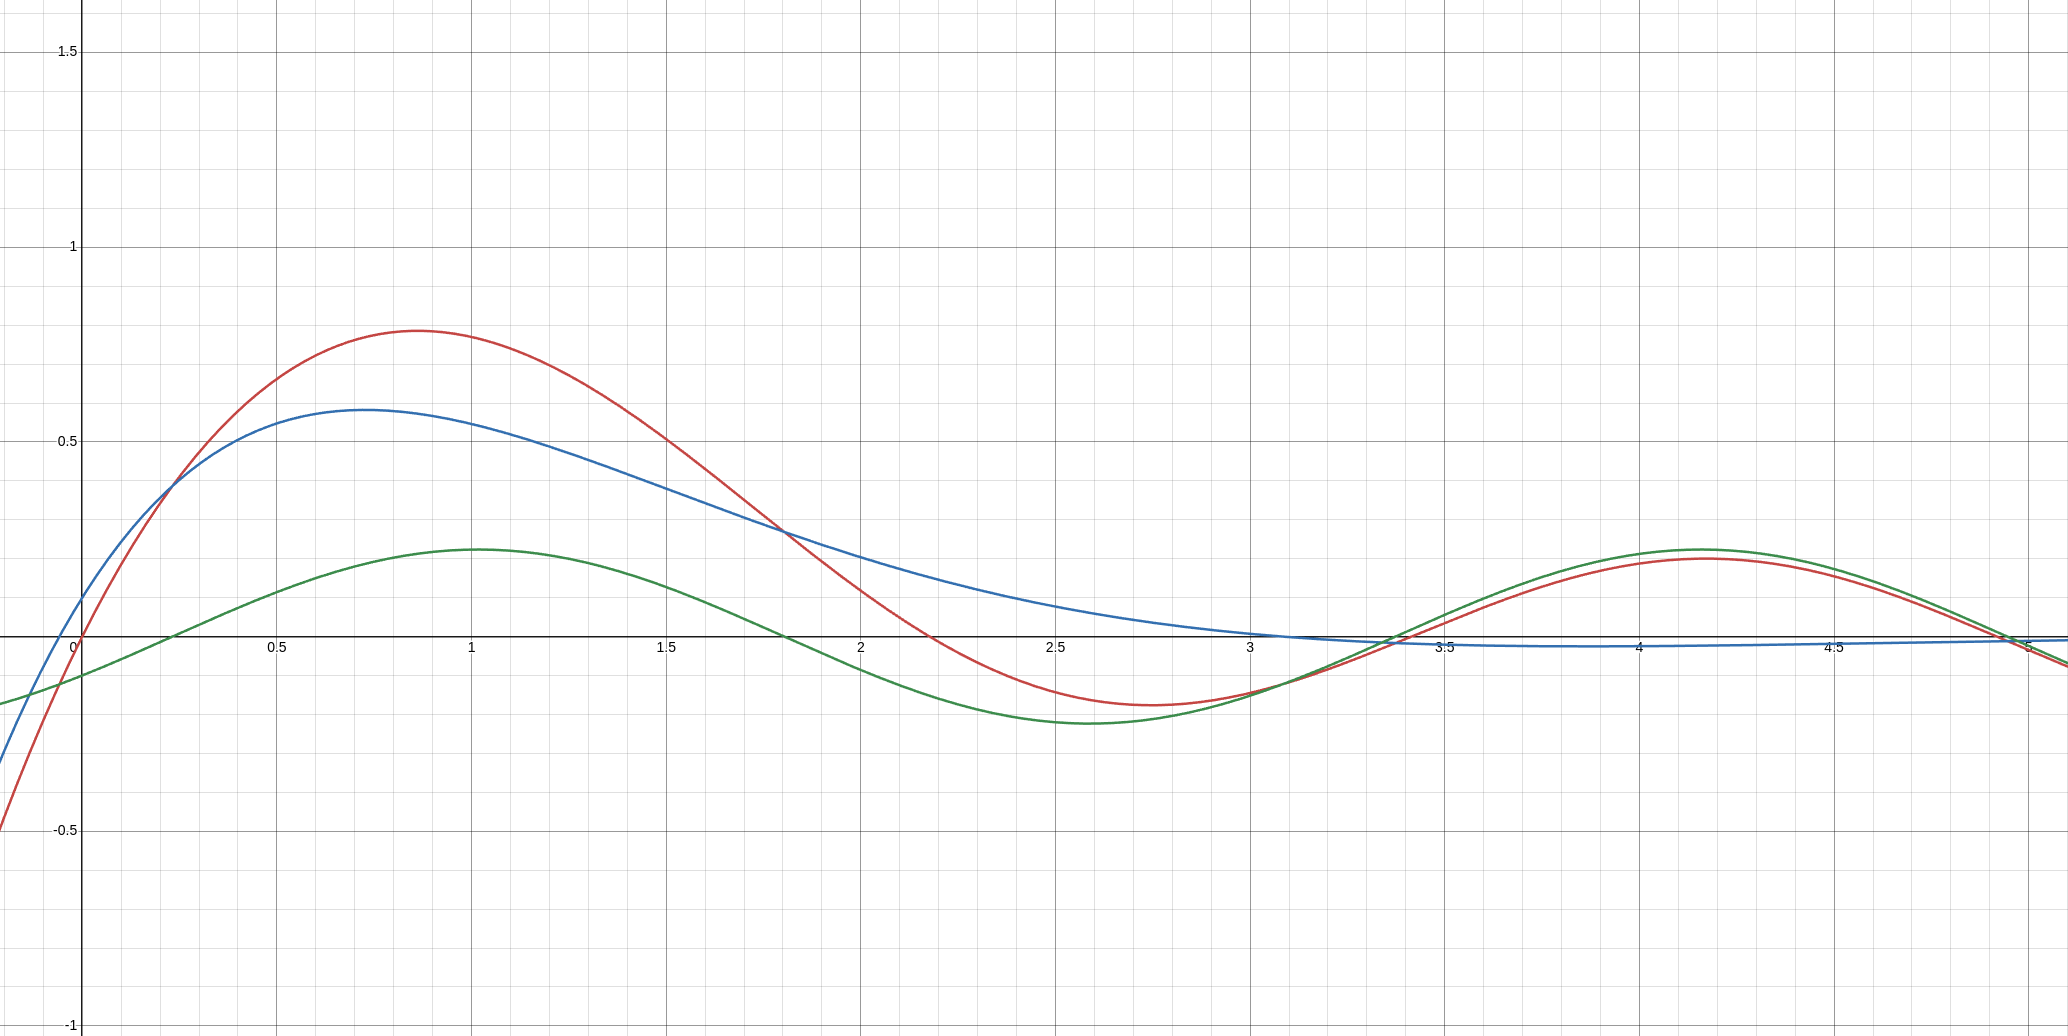
\includegraphics[width=10cm]{img/driven_damped} \\
              \small{The red line is the overall solution. The blue line is the transient one, while the green line is the steady-state one.}
          \end{center}

    \item \begin{enumerate}
              \item For resonance to occur, $\omega=\omega_0$. In this case, $\omega=2$, so $\omega_0=2$ as well and $c=\omega_0^2=\boxed{4}$.

                    In this case, our general solution is
                    \[x=C_1\cos(\omega_0t)+C_2\sin(\omega_0t)-\frac{A}{2\omega_0}t\cos(\omega t)\]
                    Solving for initial conditions, we have
                    \begin{gather*}
                        x(0)=C_1=1 \rightarrow C_1=1 \\
                        x'(0)=C_2\omega_0-\frac{1}{4}=0 \rightarrow C_2=\frac{1}{8}
                    \end{gather*}
                    and our final specific solution is
                    \[x=\cos(2t)+\frac{1}{8}\sin(2t)-\frac{t}{4}\cos(2t)\]
              \item Let's first convert the given frequency into an angular frequency: $0.1 \frac{1}{s}=0.1 \cdot 2\pi \frac{rad}{s}$

                    Now, we must solve
                    \[\frac{|\omega_0-\omega|}{2}=0.1 \cdot 2\pi \rightarrow \omega_0-\omega=\pm 0.1 \cdot 4\pi\]
                    $\omega=2$, so $\omega_0=(\pm 0.4 \cdot \pi)+2$ and by extension we have
                    \[c=\omega_0^2\approx \boxed{0.553\text{ or }10.605}\]
          \end{enumerate}
    \item \begin{enumerate}
              \item Assume that the solution takes the form $y=ate^t$. Then,
                    \begin{gather*}
                        y'=a(t+1)e^t \\
                        y''=a(t+2)e^t \\
                        y''-y=2ae^t=e^t \\
                        a=\frac{1}{2}
                    \end{gather*}
                    Thus, $\boxed{y_p=\frac{t}{2}e^t}$.
              \item For the homogeneous equation, we solve the characteristic polynomial first.
                    \[\lambda^2-1=0 \therefore \lambda=\pm 1 \therefore y_1=e^{-\lambda}, y_2=e^\lambda\]
                    Now, with variation of parameters, we assume $y_p=v_1y_1 + v_2y_2$.
                    It remains to solve the system of equations
                    \begin{gather*}
                        v_1'e^t+v_2'e^{-t}=0 \\
                        v_1'e^t-v_2'e^{-t}=e^t
                    \end{gather*}
                    Adding the first equation to the second, we get $2v_1'e^t=e^t$ and by extension $v_1'=\frac{1}{2}$.
                    Plugging it back in, we have $v_2'=-\frac{e^{2t}}{2}$.

                    Integrating these two expressions, we get $v_1=\frac{t}{2}$ and $v_2=-\frac{e^{2t}}{4}$.
                    Thus, our particular solution is
                    \[y_p=e^t\left(\frac{t}{2}-\frac{1}{4}\right)\]
          \end{enumerate}
\end{enumerate}
\end{document}
